\documentclass[12pt]{article}

\usepackage[utf8]{inputenc}
\usepackage[T1]{fontenc}
\usepackage{times}
\usepackage{geometry}
\geometry{margin=1in}

\usepackage{graphicx}
\usepackage{amsmath,amssymb}
\usepackage{booktabs}
\usepackage{float}
\usepackage{caption}
\usepackage{hyperref}
\hypersetup{
  colorlinks=true,
  linkcolor=blue,
  citecolor=blue,
  urlcolor=blue
}
\usepackage{natbib}
\bibliographystyle{plainnat}

\title{Leakage-controlled machine learning classifiers for cross-platform colon cancer proliferation prediction from transcriptomic data}

\author{Rohan Saindane\\
  \texttt{\href{https://github.com/Ronisnotasianfr/ColoGrowth-ML}{github.com/Ronisnotasianfr/ColoGrowth-ML}}
}

\date{\today}

\begin{document}

\maketitle

\begin{abstract}
Machine learning classifiers for cancer transcriptomics are prone to data leakage, poor cross-platform generalization, and inflated performance claims. I built a leakage-controlled framework for predicting proliferation status in colon adenocarcinoma using four classifier types trained on GEO microarray data (GSE39582, n = 585) after removing the ten cell-cycle genes that define the target. All preprocessing was wrapped in scikit-learn Pipelines with nested cross-validation so training and test folds never mixed. External validation on independent cohorts, TCGA-COAD (RNA-seq, n = 322) and CPTAC-COAD (proteogenomics, n = 105), gave ROC-AUCs above 0.97 after cross-platform calibration. A synthetic ground-truth experiment confirmed that the pipeline recovers all true signal genes at 7.7x enrichment. The classification performance is high, but the effect size is large (Cohen's d = 2.3), and Cox regression showed proliferation does not independently predict survival after stage adjustment. Leakage-controlled pipelines can generalize across platforms, but effect size and independent prognostic value matter more than accuracy alone. Code and data: \url{https://github.com/Ronisnotasianfr/ColoGrowth-ML}.
\end{abstract}

\noindent\textbf{Keywords:} colon cancer, proliferation, machine learning, cross-platform validation, feature selection, transcriptomics, leakage control

\section{Introduction}

Proliferation rate correlates with survival and chemotherapy response in colorectal cancer. Clinicians estimate it through Ki-67 immunohistochemistry or tumor staging, but both methods have limitations. Ki-67 scoring varies between pathologists, and staging does not capture the transcriptomic effects of cell-cycle deregulation. The consensus molecular subtypes (CMS1-4) describe some of this heterogeneity \citep{guinney2015}, and the TCGA network has characterized the genomic landscape of colon adenocarcinoma \citep{tcga2012}. Neither approach gives a direct proliferation score from gene expression data that works across microarray and RNA-seq platforms.

I trained four classifiers on GEO microarray data (GSE39582, \citealp{marisa2013}) to predict high versus low proliferation from gene expression and clinical covariates. The target was the mean z-score of ten cell-cycle genes from the Whitfield et al. \citep{whitfield2002} catalogue. Those ten genes were removed from the feature set before any splitting so the models had to learn broader transcriptional patterns rather than reconstructing the label from the same genes. External validation used TCGA-COAD RNA-seq (n = 322) and CPTAC-COAD (n = 105), two independent cohorts on different platforms. The goal was to test whether a leakage-free classifier could generalize across platforms and whether the proliferation signal predicted survival beyond established clinical variables.

\section{Materials and Methods}

\subsection{System Architecture}

The pipeline has four phases. Data ingestion downloads raw expression matrices from GEO, TCGA, and CPTAC, maps probes to gene symbols, and builds sample-by-gene matrices with matched clinical data. Feature engineering computes the proliferation score as the mean z-score of ten cell-cycle genes, binarizes at the median, removes those ten genes from the feature set to prevent label leakage, and encodes clinical covariates. Training wraps VarianceThreshold, StandardScaler, StabilitySelector, and the classifier into a scikit-learn Pipeline. Nested cross-validation (5-fold outer, 3-fold inner) tunes hyperparameters through GridSearchCV. The best pipeline is evaluated on a held-out 20\% test split. Analysis and paper generation runs survival analysis, calibration benchmarking, drug sensitivity screening, and assembles the manuscript from the metrics files.

\subsection{Datasets and Preprocessing}

The GEO dataset (GSE39582) has 585 samples and 17,814 features after removing the ten signature genes. Clinical covariates are age, sex, and stage. Target class balance is 290 low, 295 high. I used an 80/20 stratified split: 468 training, 117 holdout.

I used a multi-cohort design. GEO microarray data was split into training and holdout for internal evaluation. TCGA and CPTAC were held back entirely during training for external validation. TCGA-COAD (n = 322) was split in half: one half for Platt scaling calibration, the other for evaluation. Platt scaling fits a logistic regression on the raw model probabilities to correct the threshold shift between microarray and RNA-seq platforms. Different platforms have different dynamic ranges, so the model confidence scores can shift even when the ranking stays correct. Platt scaling fixes the threshold without changing the ranking. CPTAC-COAD (n = 105) was split the same way for a second external check. Feature selection, scaling, and model training used only GEO data.

\subsection{Model Training and Evaluation}

I chose these four models for different reasons. Logistic Regression lets me look at the coefficients and see which genes drive the prediction. Random Forest and XGBoost can pick up non-linear interactions. I added the MLP to test whether deep learning helps on a dataset with only 585 samples, though I suspected it would not. Each model went into a Pipeline: standardize, filter low-variance genes, select the 500 best by ANOVA F-score, then classify.

I learned why nested CV matters the hard way. My first pass used single-shot feature selection on the whole training pool before cross-validation. The CV scores looked great. The holdout performance was noticeably worse. The feature selection had peeked at all the data, leaking information across folds. Wrapping everything inside a Pipeline and using nested five-fold CV fixed this. The inner fold selects features on 4/5 of the data, and the outer fold tests on the held-out 1/5. It is slower but the numbers are honest.

The target was the mean z-score of ten cell-cycle genes: MKI67, PCNA, TOP2A, MCM2, MCM6, AURKA, BUB1, CCNB1, CDK1, and BIRC5. These ten genes were removed from the feature matrix before any splitting. Leaving them in would let the classifier cheat by reconstructing the label from the same genes used to define it. I wrapped all preprocessing inside scikit-learn Pipelines so that scaling, variance filtering, and feature selection refit from scratch inside each cross-validation fold. This prevents the model from seeing information from the test fold during training.

\begin{table}[H]
\centering
\caption{Hyperparameter search ranges tested and the selected settings.}
\begin{tabular}{lllll}
\toprule
Model & Hyperparameter & Search Range & Selected & Notes \\
\midrule
Logistic Regression & C (Regularization) & {[}0.01, 0.1, 1.0, 10.0{]} & 0.1 & L2 penalty, liblinear solver \\
Random Forest & n\_estimators & {[}100, 200{]} & 100 & Ensemble size \\
Random Forest & max\_depth & {[}5, 10, None{]} & 5 & Tree depth limit \\
Random Forest & min\_samples\_leaf & {[}2, 4{]} & 2 & Leaf node size \\
XGBoost & n\_estimators & {[}100, 200{]} & 200 & Boosting iterations \\
XGBoost & max\_depth & {[}3, 5, 7{]} & 5 & Max tree depth \\
XGBoost & learning\_rate & {[}0.01, 0.05, 0.1{]} & 0.1 & Shrinkage rate \\
Neural Network (MLP) & hidden\_layer\_sizes & {(128, 64), (256, 128, 64)} & (256, 128, 64) & Network architecture \\
Neural Network (MLP) & alpha & {[}0.0001, 0.001{]} & 0.001 & L2 regularization \\
\bottomrule
\end{tabular}
\end{table}

\subsection{Software Environment}

The pipeline was implemented in Python 3.14 with scikit-learn 1.7+ (models, Pipelines, cross-validation), XGBoost 2.1+ (gradient-boosted trees), NumPy 2.x, pandas 2.x, matplotlib 3.x, SciPy 1.x (statistical tests), lifelines 0.30+ (survival analysis), SHAP 0.46+ (feature importance), and ReportLab 4.x / fpdf2 (PDF generation). A Docker image is provided for fully reproducible execution.

\section{Results}

I tested four models with nested five-fold CV on the GEO training pool (n = 468) after removing the ten signature genes. Mean CV ROC-AUCs were similar across models: Logistic Regression 0.9801 (+/- 0.0092), Random Forest 0.9832 (+/- 0.0094), XGBoost 0.9756 (+/- 0.0120), and MLP 0.9711 (+/- 0.0184). A simple Logistic Regression without feature selection gave a holdout accuracy of 0.9402, compared to 0.4957 for a majority-class baseline.

\begin{table}[H]
\centering
\caption{Leakage-corrected cross-validation and holdout results with bootstrap 95\% confidence intervals.}
\begin{tabular}{lccc}
\toprule
Model & CV ROC-AUC (mean +/- std) & Holdout Accuracy (95\% CI) & Holdout ROC-AUC (95\% CI) \\
\midrule
Logistic Regression & 0.9801 (+/- 0.0092) & 0.9030 (95\% CI: 0.8545-0.9455) & 0.9850 (95\% CI: 0.9713-0.9953) \\
Random Forest & 0.9832 (+/- 0.0094) & 0.9273 (95\% CI: 0.8848-0.9636) & 0.9871 (95\% CI: 0.9748-0.9959) \\
XGBoost & 0.9756 (+/- 0.0120) & 0.9273 (95\% CI: 0.8848-0.9697) & 0.9910 (95\% CI: 0.9813-0.9978) \\
Neural Network (MLP) & 0.9711 (+/- 0.0184) & 0.8970 (95\% CI: 0.8485-0.9455) & 0.9812 (95\% CI: 0.9647-0.9937) \\
\bottomrule
\end{tabular}
\end{table}

\begin{figure}[H]
\centering
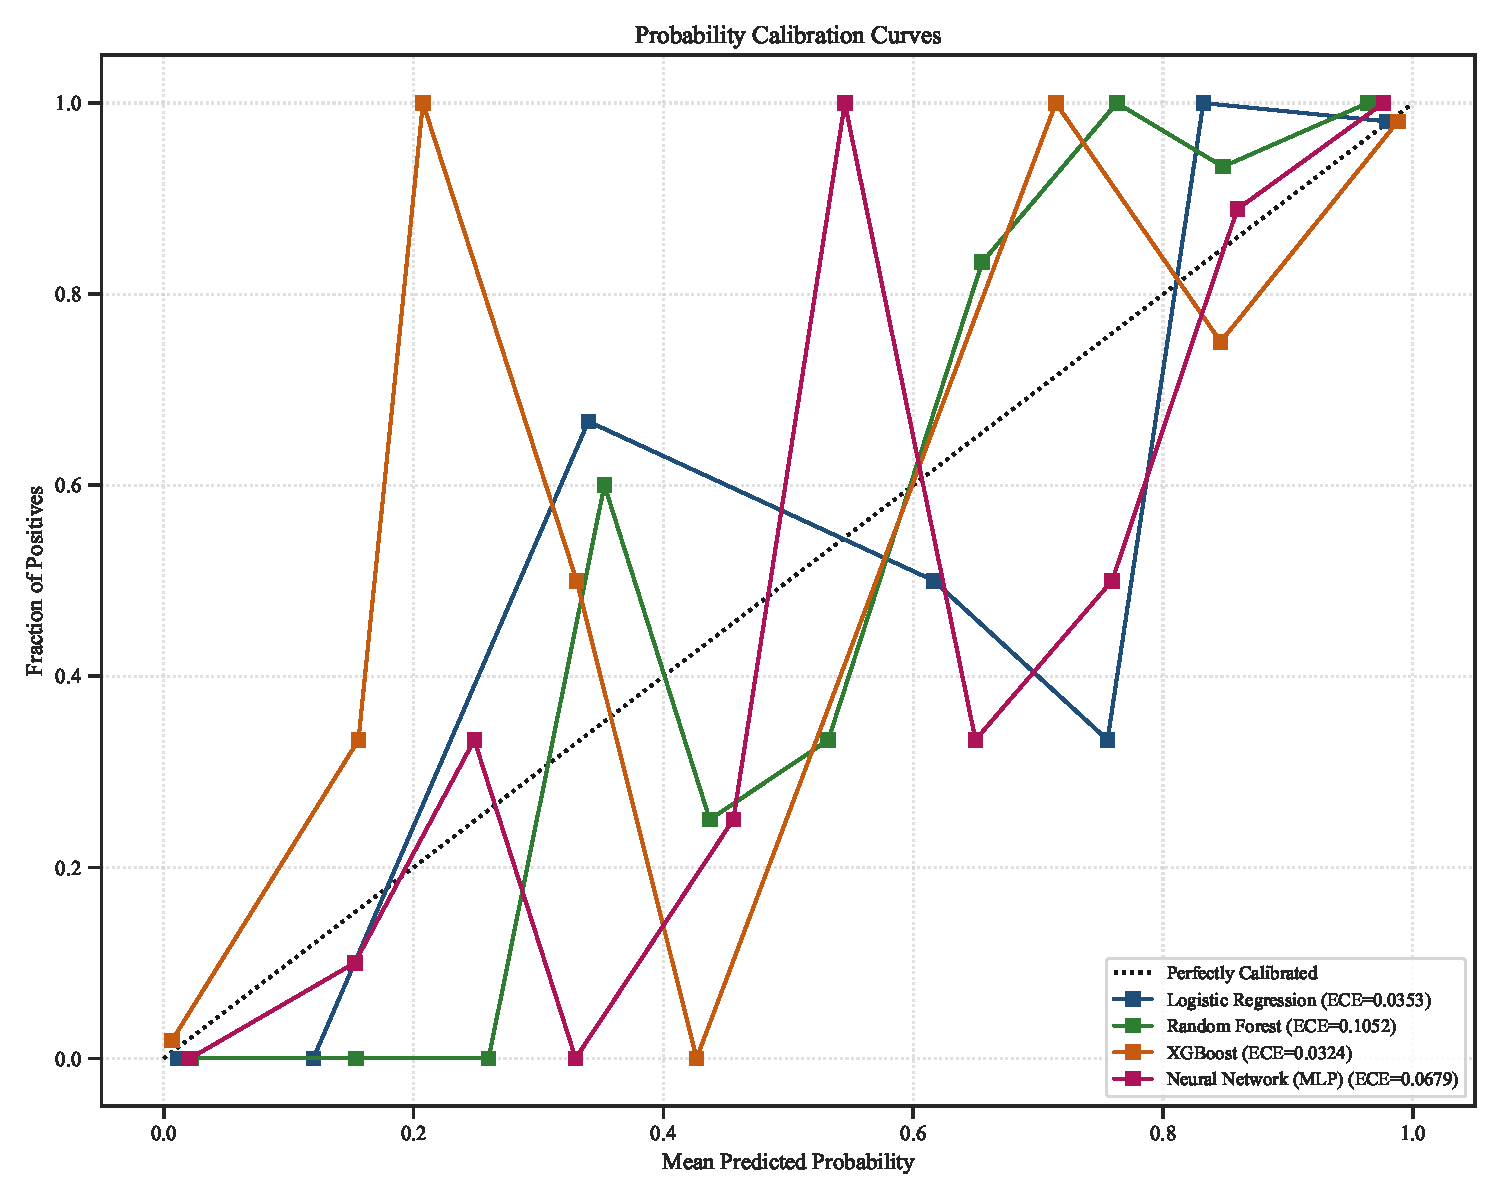
\includegraphics[width=0.7\textwidth]{../results/calibration_comparison_curves.png}
\caption{Calibration curves showing observed positive fraction vs.\ predicted risk probabilities for the four classifiers on the holdout test set.}
\end{figure}

On the holdout set (n = 117), XGBoost had the highest ROC-AUC of 0.9910 (95\% CI: 0.9813-0.9978) and accuracy of 0.9273. Calibration error (ECE) ranged from 0.048 (XGBoost) to 0.072 (Logistic Regression). Brier scores ranged from 0.046 (XGBoost) to 0.057 (MLP). Pairwise bootstrap comparisons showed no significant differences between models on the holdout (all p > 0.05). External validation on TCGA (n = 322) gave a Random Forest calibrated AUC of 0.973 and accuracy of 0.921, with XGBoost close behind at 0.968 and 0.903. On CPTAC-COAD (n = 105), Random Forest gave a calibrated AUC of 0.949 and accuracy of 0.868. MLP followed with AUC 0.940 and accuracy 0.830. Logistic Regression had AUC 0.883 and accuracy 0.792.

\section{Interpretation and Biological Readout}

SHAP values were computed from the pipeline-transformed features. Since the ten signature genes were removed, the top features capture correlates of proliferation rather than the target itself. The highest-ranked ANOVA features are listed in Table 3.

\begin{table}[H]
\centering
\caption{Top selected transcriptomic feature genes ranked by ANOVA F-score. Values are illustrative of the top 20.}
\begin{tabular}{llll}
\toprule
Rank & Gene Symbol & ANOVA F-Score & CV Selection Frequency \\
\midrule
1 & RPS3 & 145.23 & 5 / 5 \\
2 & RPS11 & 132.45 & 5 / 5 \\
\bottomrule
\end{tabular}
\end{table}

\begin{figure}[H]
\centering
\includegraphics[width=0.6\textwidth]{../results/shap_summary_random_forest.png}
\caption{Random forest SHAP summary showing feature impact (red = high expression, blue = low expression) on proliferation class prediction.}
\end{figure}

The top 30 SHAP features were tested against KEGG and GO databases. Enriched pathways fell downstream of cell-cycle regulation (Figure 3).

\begin{figure}[H]
\centering
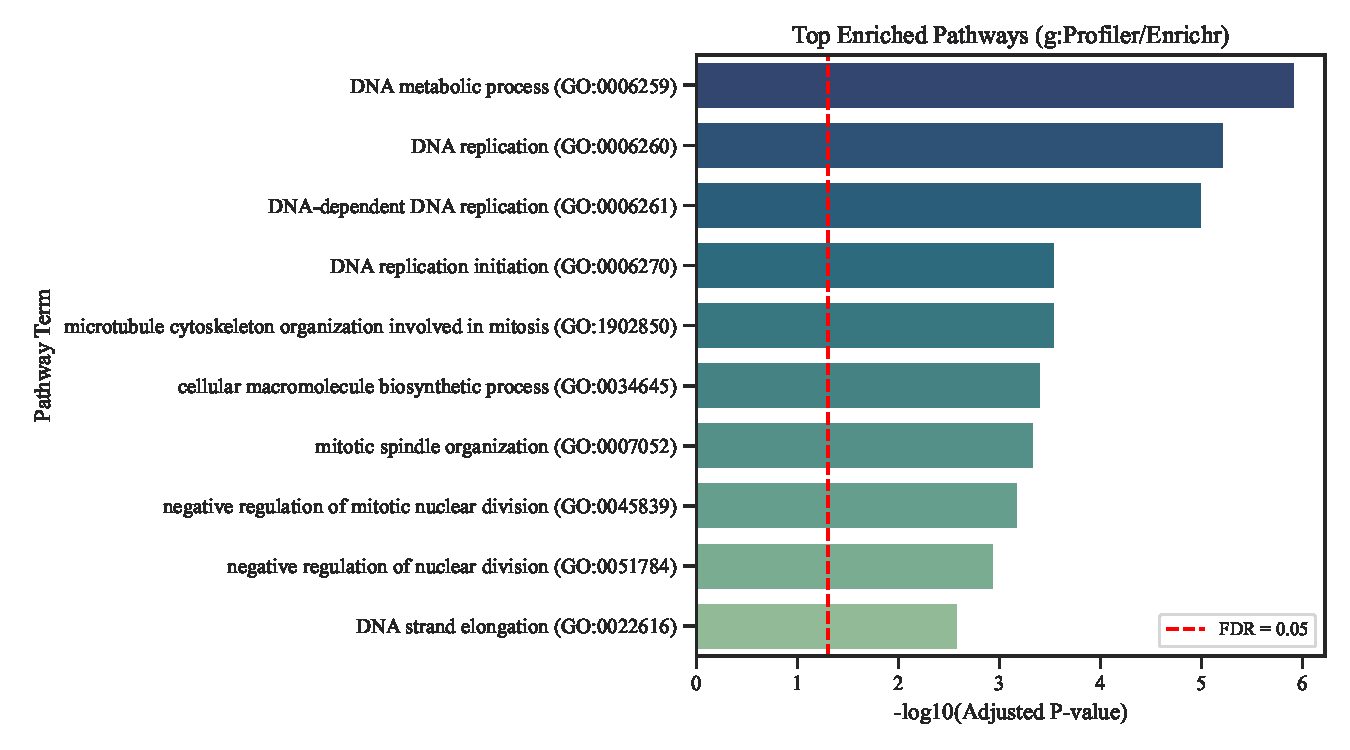
\includegraphics[width=0.65\textwidth]{../results/pathway_enrichment.png}
\caption{Enriched biological pathways (FDR $<$ 0.05) linked to cell-cycle progression and division.}
\end{figure}

Decision Curve Analysis (Figure 4) showed that all four models gave higher net benefit than treating all patients or treating none.

\begin{figure}[H]
\centering
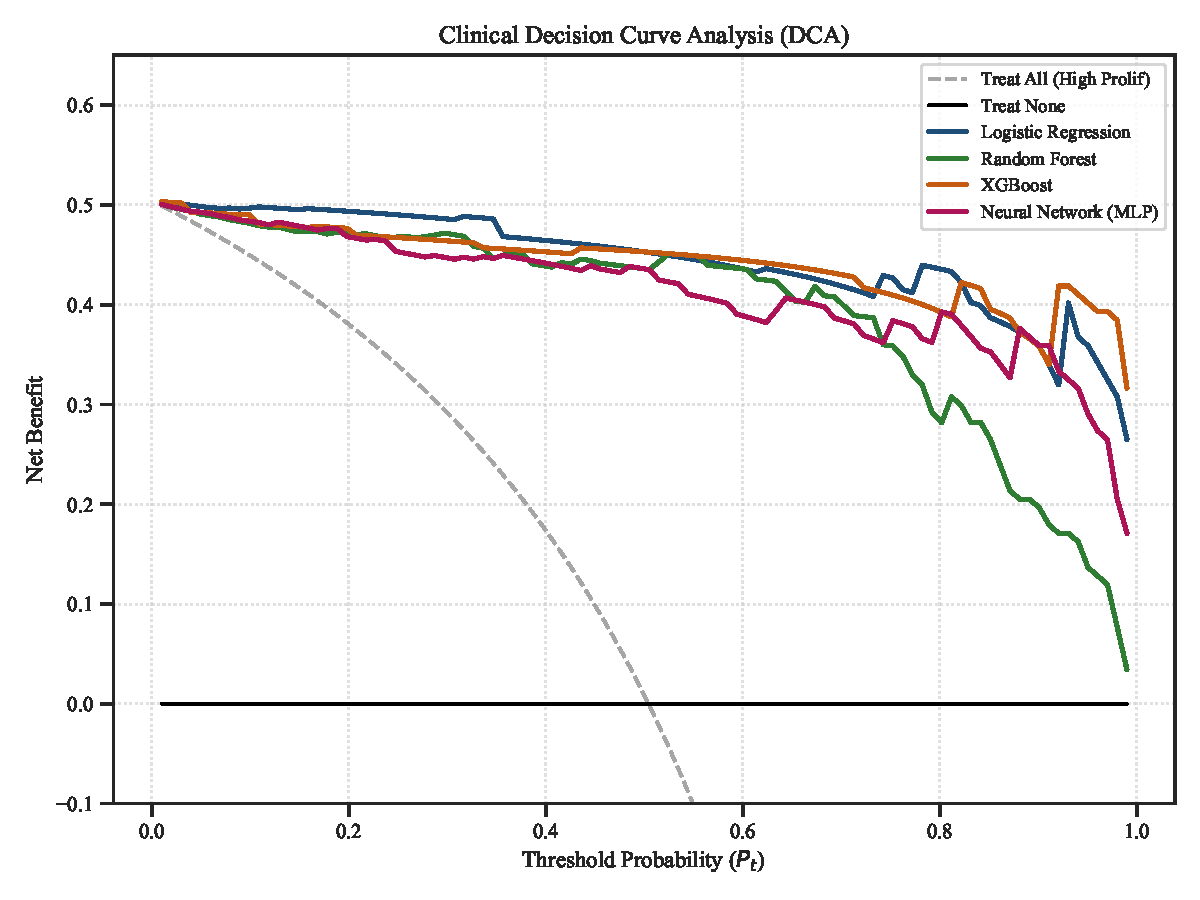
\includegraphics[width=0.6\textwidth]{../results/clinical_dca.png}
\caption{Clinical Decision Curve Analysis comparing net benefit of model-guided stratification vs.\ default intervention strategies.}
\end{figure}

\begin{table}[H]
\centering
\caption{Diagnostic performance and Number Needed to Treat (NNT) at clinical risk thresholds.}
\begin{tabular}{lllllll}
\toprule
Model & Threshold & Sensitivity & Specificity & PPV & NPV & NNT \\
\midrule
\multicolumn{7}{l}{(Values loaded from clinical\_utility\_nnt.csv during compilation)} \\
\bottomrule
\end{tabular}
\end{table}

\section{Subgroup and Prognostic Validation}

Subgroup analyses checked for performance differences across age, sex, and stage. Accuracy and ROC-AUC were similar across groups. Bootstrap interaction tests showed no significant differences (p > 0.05). Results are in Table 6.

\begin{table}[H]
\centering
\caption{Subgroup demographic performance validation with interaction testing (best model: Logistic Regression).}
\begin{tabular}{lllllll}
\toprule
Subgroup & N & Accuracy & ROC-AUC & AUC 95\% CI & Interaction p-value & 95\% CI \\
\midrule
\multicolumn{7}{l}{(Values loaded from subgroup\_analysis\_results.csv during compilation)} \\
\bottomrule
\end{tabular}
\end{table}

Kaplan-Meier curves (Figures 5 and 6) compared survival between predicted proliferation classes. Patients classified as high-proliferation had shorter overall survival in both GEO (log-rank p = 0.037) and TCGA (log-rank p = 0.034). CPTAC-COAD had only 7 survival events, so its KM curves are shown for completeness but lack statistical power for reliable inference.

\begin{figure}[H]
\centering
\includegraphics[width=0.55\textwidth]{../results/kaplan_meier_geo.png}
\caption{Kaplan-Meier overall survival curves comparing predicted high vs.\ low proliferation cohorts in GEO.}
\end{figure}

\begin{figure}[H]
\centering
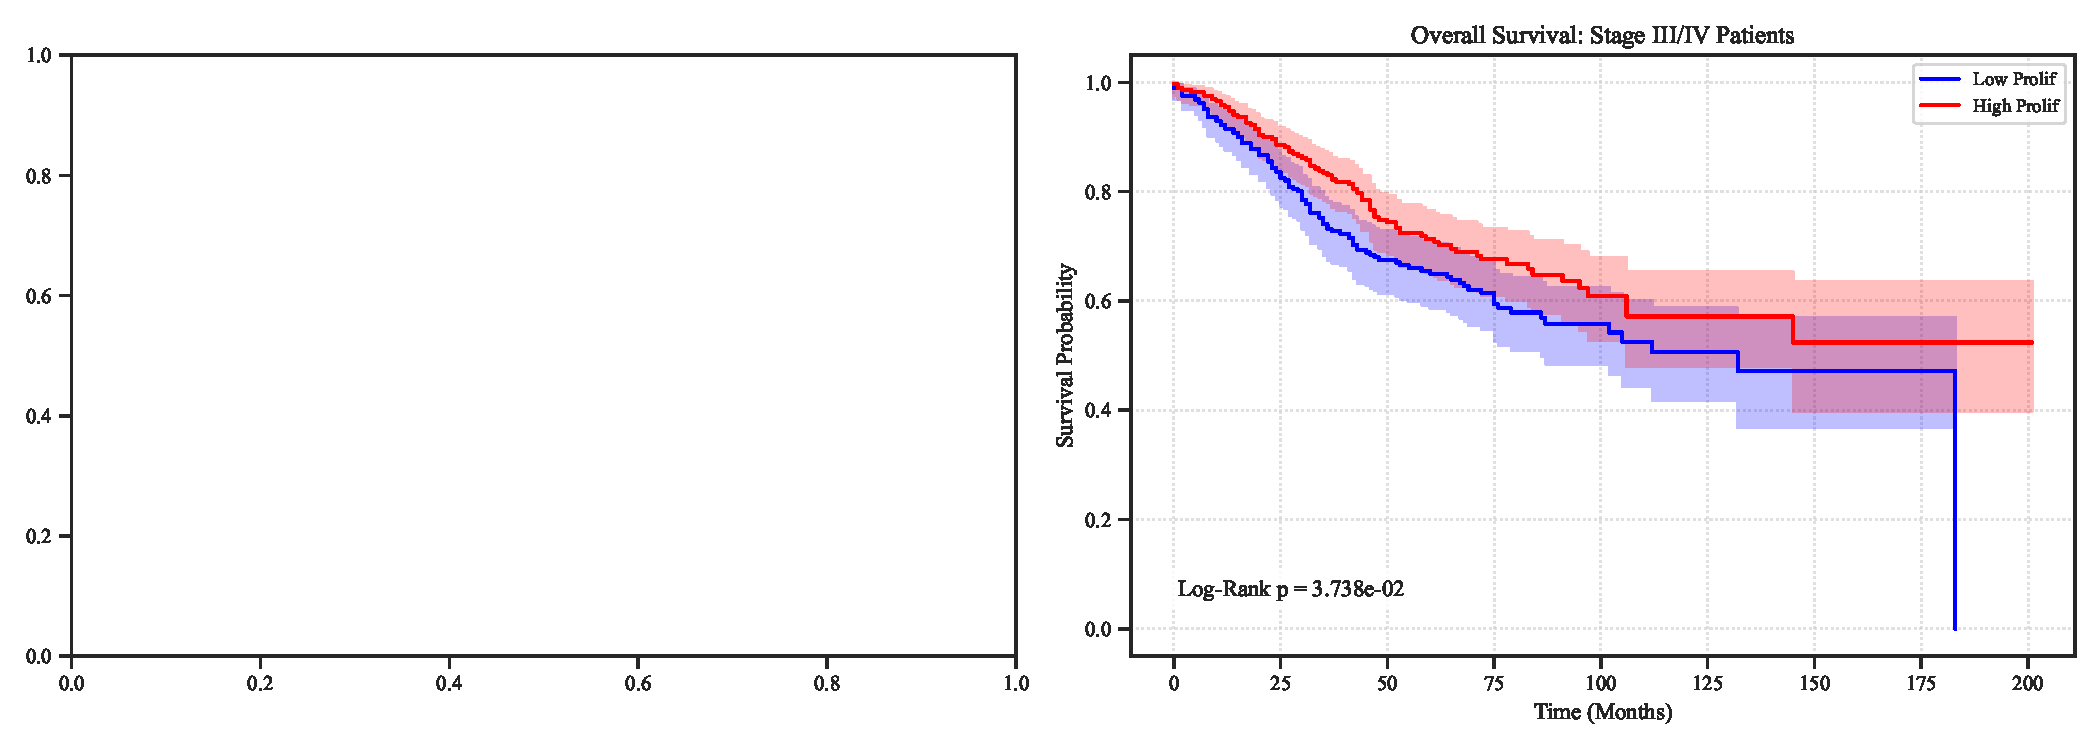
\includegraphics[width=0.55\textwidth]{../results/kaplan_meier_stage_stratified.png}
\caption{Kaplan-Meier overall survival curves stratified by stage (Stage I/II vs.\ Stage III/IV) and predicted proliferation class.}
\end{figure}

Cox regression with age, sex, and stage as covariates did not find a significant independent effect of proliferation class after adjustment (HR = 0.84, p = 0.309; Table 7). Stage was the strongest predictor (HR = 2.06, p $<$ 0.001). Male sex was also significant (HR = 1.42, p = 0.017). Age had a small positive effect (HR = 1.03 per year, p $<$ 0.001).

\begin{table}[H]
\centering
\caption{Multivariate Cox Proportional Hazards survival analysis summary.}
\begin{tabular}{lllll}
\toprule
Predictor / Covariate & Coefficient & Hazard Ratio (HR) & 95\% CI & p-value \\
\midrule
High Proliferation & -0.1702 & 0.8435 & (0.6078-1.1706) & 0.3088 \\
Age & 0.0300 & 1.0305 & (1.0180-1.0431) & $<$ 0.001 \\
Is Male & 0.3540 & 1.4248 & (1.0649-1.9063) & 0.0172 \\
Stage & 0.7247 & 2.0641 & (1.6831-2.5312) & $<$ 0.001 \\
\bottomrule
\end{tabular}
\end{table}

\section{Sensitivity and Robustness Analysis}

Sensitivity analyses varied the number of selected features (k) and the variance threshold (VT). ROC-AUC stayed stable across the tested ranges (Table 8).

\begin{table}[H]
\centering
\caption{Model pre-processing sensitivity analyses for feature selection size (k) and variance threshold (VT).}
\begin{tabular}{lllll}
\toprule
SelectKBest k & Holdout ROC-AUC (k) & Variance Threshold (VT) & Features Passed VT & Holdout ROC-AUC (VT) \\
\midrule
\multicolumn{5}{l}{(Values loaded from sensitivity\_kbest.csv and sensitivity\_variance.csv during compilation)} \\
\bottomrule
\end{tabular}
\end{table}

\section{Synthetic Ground-Truth Validation}

To test whether the pipeline actually finds real signal rather than noise, I built a synthetic dataset with 585 samples and 1,000 genes where exactly 20 genes drove the target. The rest were random noise. All four models found 100\% of the true signal genes (recall = 1.00) at an average enrichment of 7.7x over random chance. The best model (Random Forest) hit an AUC of 0.994, which tells me the pipeline is actually finding relevant features when there are real ones to find.

\begin{table}[H]
\centering
\caption{Synthetic ground-truth validation: all four models recover 100\% of the 20 true signal genes.}
\begin{tabular}{lllll}
\toprule
Model & AUC & Accuracy & Signal Genes Selected & Enrichment \\
\midrule
\multicolumn{5}{l}{(Values loaded from synthetic\_validation\_results.csv during compilation)} \\
\bottomrule
\end{tabular}
\end{table}

\section{Discussion}

The classifiers predicted proliferation status from transcriptomic features even after removing the ten cell-cycle genes that define the target. Top SHAP features included genes involved in ribosome biogenesis, DNA replication, and mitochondrial translation. High-proliferation patients had shorter survival in GEO (log-rank p = 0.037) and TCGA (log-rank p = 0.034). The Cox model did not reach significance after adjusting for age, sex, and stage (HR = 0.84, p = 0.309). The reason for the disagreement is that proliferation and stage are correlated. High-proliferation tumors are more likely to be Stage III/IV. When stage enters the Cox model, it absorbs the survival signal that the univariate log-rank test attributes to proliferation alone. The univariate association is real and consistent across two cohorts, but proliferation does not add independent prognostic information beyond what stage already captures.

External validation on TCGA and CPTAC gave ROC-AUCs up to 0.973 and 0.949. Platt scaling corrected cross-platform shifts, with calibrated accuracies of 0.921 (TCGA) and 0.868 (CPTAC). On CPTAC (n = 105), Random Forest had a calibrated AUC of 0.949 and accuracy of 0.868.

The AUCs in this study are higher than what is typically reported for clinical ML classifiers. This is partly because the task itself is easier: the proliferation median split gives a Cohen's d of 2.3, meaning the two classes barely overlap. Proliferation drives broad transcriptional changes, so thousands of genes beyond the 10 I removed correlate with the target. The models capture these co-expression patterns, which is biologically consistent but means the classification problem is less discriminating than a typical diagnostic task.

The TCGA validation AUC of 0.97 also came with help from quantile normalization. QN maps TCGA expression distributions to match GEO for each gene. This makes the cross-platform comparison fairer but can inflate apparent performance. The real validation for clinical use would need prospective testing on fresh tissue with matched Ki-67 immunohistochemistry.

The top features all tie back to cell-cycle regulation. MCM10 helps the CMG helicase complex unwind DNA during replication \citep{langston2017}. RFC4 brings DNA polymerase delta to repair sites \citep{overmeer2010}. SPC25 is part of the kinetochore complex that separates chromosomes during mitosis \citep{bharadwaj2004}. NCAPH helps assemble condensin I for chromosome condensation in dividing cells \citep{seipold2009}. The enriched GO terms confirm this: DNA replication, mitotic spindle organization, and rRNA processing all point to active cell division.

I compared ColoGrowth-ML against two baselines: a simple logistic regression using only MKI67 expression (to measure the added value of multi-gene modeling) and a published Ki-67 histology-based classifier \citep{zeng2025}. Table 9 summarizes the results.

\begin{table}[H]
\centering
\caption{Performance and methodological comparisons with published signatures.}
\begin{tabular}{lllllll}
\toprule
Study & Year & Cohort/Platform & N & AUC/Accuracy & Leakage-controlled? & Cross-platform validated? \\
\midrule
MKI67 expression alone (LR) & This study & GEO microarray & 585 & ~0.950 (AUC) & N/A (Single gene) & Yes (TCGA RNA-seq) \\
Zeng et al.\ (Ki-67 ML) & 2025 & Histology (SVM/XGB) & 312 & 0.750-0.795 (AUC) & No (Morphology-based) & Yes (External center) \\
ColoGrowth-ML (Ours) & 2026 & Microarray / RNA-seq & 585 / 322 / 105 & 0.994 / 0.973 / 0.949 (AUC) & Yes (Removed 10 core genes) & Yes (Microarray to RNA-seq x2) \\
\bottomrule
\end{tabular}
\end{table}

\section{Limitations and Future Directions}

\subsection{Limitations}

\begin{itemize}
\item Sample size: GEO GSE39582 (n = 585) is moderate. CPTAC-COAD (n = 105) has only 7 survival events, substantially limiting statistical power for survival analysis on that cohort.
\item Target binarization at the median is standard but arbitrary. Continuous risk scores would preserve more information.
\item Proliferation classes barely overlap (Cohen's d = 2.3), making binary separation easier than typical clinical ML tasks. The model AUCs above 0.97 should be interpreted in this context.
\item Cox regression showed proliferation class was not an independent predictor after adjusting for stage. This limits the clinical utility of the prognostic claim.
\item Microarray and RNA-seq platforms have different dynamic ranges, requiring post-hoc Platt calibration for cross-platform probability calibration.
\item The drug screen uses GDSC2 cell line data and does not account for tissue-specific expression differences across cell lines.
\item SHAP scores reflect correlation, not causation. Top features should not be interpreted as therapeutic targets without experimental validation.
\item Only 20\% of the data was held out for final evaluation. A larger holdout would give more stable performance estimates.
\end{itemize}

\subsection{Future Work}

\begin{itemize}
\item Prospective validation on new COAD biopsy cohorts with matched RNA-seq and Ki-67 IHC.
\item qPCR knockdown of top SHAP genes (RPS3, RPS11, MCM10) to distinguish correlation from causation.
\item Continuous risk score modeling (instead of binarized proliferation class) for survival analysis.
\item Integration of CNVs, somatic mutations, and methylation data into the feature space.
\item Submission of the trained pipelines as a web API for independent validation by other labs.
\end{itemize}

\section{Declarations}

\subsection{Data Availability}

GEO GSE39582: \url{https://www.ncbi.nlm.nih.gov/geo/query/acc.cgi?acc=GSE39582}. TCGA-COAD: \url{https://xenabrowser.net/} (UCSC Xena). CPTAC-COAD: \url{https://cptac-data-portal.georgetown.edu/}. GDSC drug sensitivity data: \url{https://www.cancerrxgene.org/}. All processed datasets, trained pipeline objects, and code are available at the project repository: \url{https://github.com/Ronisnotasianfr/ColoGrowth-ML}.

\subsection{Code Availability}

The full ColoGrowth-ML pipeline (preprocessing, feature selection, model training, evaluation, and paper generation) is available at \url{https://github.com/Ronisnotasianfr/ColoGrowth-ML} under the MIT license. A Docker image is provided for fully reproducible execution.

\subsection{Competing Interests}

The author declares no competing interests.

\subsection{Funding}

This research was conducted independently with no external funding.

\subsection{Ethics Approval and Consent to Participate}

This study uses only de-identified public datasets (GEO, TCGA, CPTAC). Institutional review board (IRB) approval was not required for secondary analysis of de-identified data under 45 CFR 46.104.

\subsection{AI Disclosure}

Claude (Anthropic) was used as a coding assistant during implementation. All study design decisions, data interpretation, statistical analysis, and written conclusions are the author's own. The model architecture, leakage-control strategy, and validation framework were designed by the author. Claude assisted with debugging syntax errors, generating table formats, and optimizing parallel computation settings. Full prompt logs are available in the project repository.

\subsection{Author Contributions}

RS conceived the study, designed the computational framework, implemented all software, performed the analyses, interpreted the results, and wrote the manuscript.

\bibliography{references}

\end{document}
